\documentclass[12pt,a4paper]{article}

% Margins.
\setlength{\oddsidemargin}{0in}
\setlength{\evensidemargin}{0in}
\setlength{\headheight}{12pt}
\setlength{\headsep}{42pt}
\setlength{\topmargin}{-54pt}
\setlength{\textwidth}{6.5in}
\setlength{\textheight}{10in}

\usepackage{amsmath}
\usepackage{float}
\usepackage{graphicx}
\usepackage[hyphens]{url}
\usepackage{hyperref}	% Clickable links to figures, references and urls.
\usepackage{datetime}
\usepackage{longtable}
\usepackage{subfigure}

% Links direct to top of figures.
\usepackage[all]{hypcap}

% Drawing.
\usepackage{pgf}
\usepackage{tikz}

% Listings for formatting code.
\usepackage{listings}
\usepackage{textcomp}
% General options.+++
\lstset{breaklines=true, basicstyle=\small\ttfamily, tabsize=4, numbers=left, stepnumber=1, frame=single, showstringspaces=false, upquote=true}
% C++ specific high-lighting. Comments are 50/50 shades of green/black and strings coloured with 60/40 red/black mixture.
\lstset{language=[ISO]C++, commentstyle=\color{green!50!black}, keywordstyle=\color{blue}, stringstyle=\color{red!60!black}}

%opening
\title{\vspace{-3cm}Physics for Engineers\\Class 21\\Electric Field Lines\\Motion of a Charged Particle in Electric Field}
\author{Attique Dawood}
\date{March 11, 2014\\[0.2cm] Last Modified: \today, \currenttime}
\begin{document}
\maketitle
\section{Announcements}
\begin{itemize}
\item None.
\end{itemize}
\section{Revision}
\begin{itemize}
\item Electric field of continuous charge distributions.
\end{itemize}
\section{Electric Field Lines}
\begin{itemize}
\item Electric field lines is a way of depicting electric field. This is an old concept and less frequently used in recent times.
\item Another way of representing electric field is to plot electric field vectors at each point in space. This is mostly used nowadays due to computing softwares that can easily plot electric fields.
\item Electric field line representation is different from vector representation because in case of vectors, length of vector gives field strength or magnitude, whereas, density (or number) of field lines give field strength.
\item If there are charges present then electric field lines will originate from positive charges and terminate at negative charges.
\end{itemize}
\section{Motion of a Charged Particle in Uniform Electric Field}
\begin{equation}
\textbf{F}=q\textbf{E}
\end{equation}
\begin{equation}
\textbf{a}=\dfrac{\textbf{F}}{m}
\end{equation}
\section{Exercises}
\noindent\textbf{Question 1 \cite[Example 23.11, page 727]{Serway}:} An electron enters the region of a uniform electric field as shown in Figure 23.26, with $v_i = 3.00 \times 10^6$ m/s and \textbf{E} = 200 N/C. The horizontal length of the plates is 0.100 m. Find
\begin{itemize}
\item Acceleration.
\item Time it leaves the field.
\item Vertical position as it leaves the field.
\end{itemize}
%\begin{figure}[H]
%\centering
%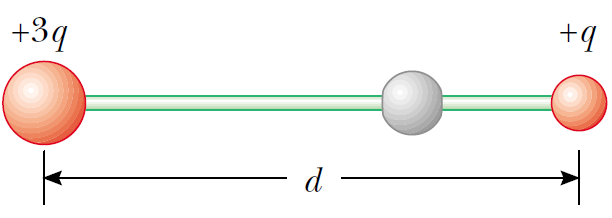
\includegraphics[scale=0.45]{FigureP23-10.png}
%\caption{Equilibrium of charge.}
%\label{Equilibrium}
%\end{figure}
%\nocite{*}
\bibliographystyle{plain}
\bibliography{PhysicsRef}
\end{document}
